\documentclass{article}
\usepackage[x11names, svgnames, rgb]{xcolor}
\usepackage[utf8]{inputenc}
\usepackage{tikz}
\usetikzlibrary{snakes,arrows,shapes}
\usepackage{amsmath}
%
%

%

%

\begin{document}
\pagestyle{empty}
%
%
%

\enlargethispage{100cm}
% Start of code
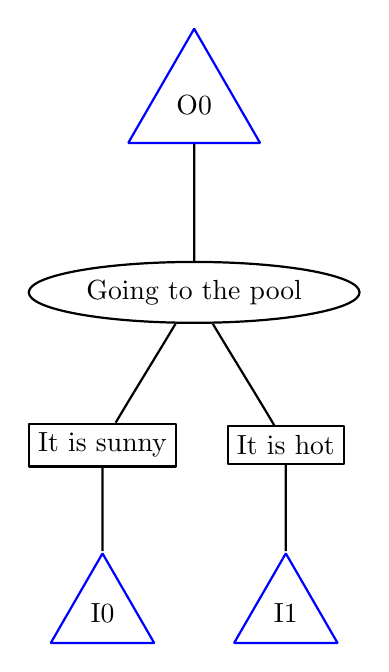
\begin{tikzpicture}[>=latex',line join=bevel,]
%%
\begin{scope}[thick]
  \node (It is sunny) at (26.5bp,77.0bp) [draw,rectangle] {It is sunny};
  \node (I0) at (26.5bp,16.5bp) [draw=blue,regular polygon, regular polygon sides=3] {I0};
  \node (It is hot) at (92.5bp,77.0bp) [draw,rectangle] {It is hot};
  \node (I1) at (92.5bp,16.5bp) [draw=blue,regular polygon, regular polygon sides=3] {I1};
  \node (Going to the pool) at (59.5bp,132.0bp) [draw,ellipse] {Going to the pool};
  \node (O0) at (59.5bp,199.5bp) [draw=blue,regular polygon, regular polygon sides=3] {O0};
\end{scope}
\begin{scope}[thick]
  \draw [] (It is sunny) ..controls (26.5bp,60.04bp) and (26.5bp,44.898bp)  .. (I0);
  \draw [] (It is hot) ..controls (92.5bp,61.133bp) and (92.5bp,45.352bp)  .. (I1);
  \draw [] (Going to the pool) ..controls (46.619bp,110.31bp) and (36.656bp,94.311bp)  .. (It is sunny);
  \draw [] (Going to the pool) ..controls (72.605bp,109.95bp) and (83.035bp,93.201bp)  .. (It is hot);
  \draw [] (O0) ..controls (59.5bp,176.95bp) and (59.5bp,155.8bp)  .. (Going to the pool);
\end{scope}
%
\end{tikzpicture}
% End of code

%
\end{document}
%



